% !TEX encoding = UTF-8
% !TEX program = pdflatex
% !TeX spellcheck = en_GB
% !BIB = biber


\documentclass[english]{article}
\usepackage{babel}
\usepackage[utf8]{inputenc}
\usepackage{graphicx}
\graphicspath{{./images/}}
\usepackage{hyperref}
\usepackage{csquotes}
\hypersetup{
    colorlinks=true, 
	linkcolor=blue, 
	filecolor=blue, 
	citecolor = black,       
	urlcolor=blue, 
}


\usepackage{biblatex}
\addbibresource{bib.bib}

\title{5G Security}
\author{Alessandro Castelli \\ ID:\@147073 \\ E-mail: castelli.alessandro@spes.uniud.it}

\begin{document}

\maketitle

\begin{abstract}
	Negli ultimi decenni, le comunicazioni wireless hanno subito una rapida
	evoluzione, alimentata dalla crescente domanda degli utenti per connessioni
	sempre più veloci, affidabili e performanti. Tra le innovazioni tecnologiche
	più rilevanti, la tecnologia 5G si è affermata come la nuova frontiera delle
	telecomunicazioni mobili, promettendo una capacità di banda superiore,
	latenze ridotte e una enorme densità di connessioni per dispositivi
	intelligenti e IoT. Tuttavia, insieme a queste straordinarie capacità,
	emergono anche nuove sfide in termini di sicurezza. Il 5G introduce una
	infrastruttura di rete più complessa e decentralizzata, aumentando il rischio
	di vulnerabilità e attacchi informatici. Questo articolo esamina i principali
	aspetti della sicurezza del 5G, evidenziando le vulnerabilità della rete e
	discutendo le soluzioni tecnologiche avanzate sviluppate per mitigare i rischi.
\end{abstract}

\clearpage

\tableofcontents
\newpage
\section{Introduzione}

La storia della comunicazione mobile è un viaggio di innovazione continua.
Tutto inizia con il 1G~\cite{dangi2021study}, negli anni '70 e '80, quando la
trasmissione dei dati era analogica. Era l'inizio, ma con grandi limiti: la
qualità era bassa, la sicurezza inesistente e le chiamate potevano essere
facilmente intercettate. Tuttavia, consentiva qualcosa di rivoluzionario per
l'epoca: la connettività mobile e i primi servizi vocali, anche se in modo
rudimentale.

Con l'arrivo del 2G nel 1991, la situazione cambiò drasticamente. La
comunicazione diventò digitale, affrontando molti dei problemi del 1G. Ora
c'era più sicurezza, efficienza e una maggiore larghezza di banda. Si aprirono
così le porte a nuovi servizi come i messaggi di testo, rendendo la
comunicazione mobile più sofisticata.

Successivamente, il 3G introdusse il concetto di banda larga mobile. Non era
più solo una questione di chiamate o messaggi, ma anche di videochiamate,
navigazione su Internet e una trasmissione dati molto più veloce. Il 3G
rappresentava una svolta, anche se soffriva ancora di problemi legati allo
spettro e alla latenza, dimostrando che la tecnologia aveva ancora margini di
miglioramento.

Quando arrivò il 4G, tra il 2009 e il 2010, il mondo della comunicazione mobile
fece un enorme balzo in avanti. Grazie a tecnologie come LTE, la velocità dei
dati aumentò significativamente, portando il mobile streaming, i giochi online
e i video in alta definizione a portata di mano ovunque. Le velocità di
download teoriche potevano raggiungere i 100 Mbps, sebbene nella pratica
fossero spesso inferiori.

Infine, con l'avvento del 5G, si entrò in una nuova era. Non si parlava più
solo di miglioramenti incrementali, ma di una rivoluzione. Il 5G promette
velocità fino a 20 Gbps~\cite{javid20225g}, una latenza ultra bassa e la
capacità di connettere miliardi di dispositivi contemporaneamente. È una
tecnologia pensata per un mondo interconnesso, dove non ci sono solo
smartphone, ma anche automobili, dispositivi IoT, smart cities e sistemi
industriali automatizzati. Il 5G è il fondamento di quella che sarà l'Internet
of Everything, dove ogni aspetto della vita quotidiana è connesso e integrato
in una rete globale.

Il \textbf{5G} rappresenta quindi l'ultima evoluzione nella tecnologia di
comunicazione mobile, portando miglioramenti significativi come
\textit{larghezza di banda elevata} e \textit{latenza estremamente bassa}.
Questa tecnologia supporta applicazioni avanzate come la realtà aumentata (AR),
la realtà virtuale (VR) e le comunicazioni ultra-affidabili a bassa latenza
(URLLC). Nel marzo 2018, il
\href{https://www.3gpp.org/technologies/5g-system-overview}{3GPP} ha rilasciato
la 15ª release degli standard di comunicazione mobile, stabilendo le basi per
il \textbf{5G}. La velocità di trasmissione di questa nuova tecnologia consente
agli utenti di usufruire di trasferimenti dati notevolmente superiori, in
particolare per applicazioni che richiedono un alto throughput, come lo
streaming video in alta definizione~\cite{javid20225g}.

La riduzione della latenza è un altro obiettivo chiave, con la previsione di
una latenza inferiore a 1 millisecondo, aprendo la strada all'uso in tempo
reale di applicazioni critiche come la telemedicina e la guida autonoma.
Inoltre, il 5G permette la connessione simultanea di un numero molto maggiore
di dispositivi rispetto alle generazioni precedenti, una caratteristica
fondamentale vista la continua crescita del mercato IoT.

Grazie a tutto questo, il 5G diventerà una base per una rete che connette non
solo persone, ma anche oggetti, dispositivi e macchine. Si sta parlando,
quindi, di un sistema che sta rivoluzionando il modo in cui immaginiamo
internet, non più solo come uno scambio di dati tra persone, ma come
un'integrazione massiccia tra esseri umani e macchine, e tra macchine stesse.

E qui entrano in gioco i tre scenari fondamentali del 5G:\@ \textbf{eMBB, mMTC
	e uRLLC}. Ognuno di questi rappresenta una sfaccettatura dell'intera visione
del 5G~\cite{Ji2018Overview}: \textbf{eMBB} è pensato per una banda larga
mobile potenziata, consentendo download rapidissimi e streaming ad altissima
qualità; \textbf{mMTC} è rivolto alla comunicazione massiva tra macchine,
essenziale per supportare l’IoT (Internet of Things); \textbf{uRLLC} invece è
cruciale per applicazioni che richiedono una latenza minima e un'affidabilità
estrema, come la telechirurgia o i veicoli autonomi. Ma quali sono le
tecnologie che effettivamente rendono possibile tutto questo? \\ \sloppy Il
3GPP ha definito più di 70 tipi di file 5G SA1 necessari a questo scopo, e le
tecnologie chiave sviluppate per il 5G includono:
\textit{\hyperlink{MIMO}{Massive MIMO}}, \textit{\hyperlink{FBMC}{filter bank
		based multicarrier (FBMC)}}, \textit{\hyperlink{FullDuplex}{Full Duplex}},
\textit{\hyperlink{UDN}{Ultra Dense networking (UDN)}},
\textit{\hyperlink{SDN}{software-defined networking (SDN)}} e
\textit{\hyperlink{NFV}{network function virtualization
		(NFV)}}~\cite{Ji2018Overview}. \\ In questo articolo verrà presentato uno
studio approfondito sulla sicurezza all'interno delle reti 5G. Nella
Sezione~\ref{sec:ThreatModel} si esamineranno gli asset, gli attaccanti e i
rischi associati a una rete 5G. La Sezione~\ref{sec:SecurityGoal} illustrerà
gli obiettivi di sicurezza che si intendono raggiungere per gli asset
identificati. Nella Sezione~\ref{sec:4} verranno analizzati i servizi di
sicurezza implementati all'interno di questa tecnologia. Infine, nella
Sezione~\ref{sec:5 } si discuteranno le potenziali vulnerabilità presenti. Per
mantenere il testo chiaro e conciso, evitando complicazioni eccessive e
approfondimenti frequenti sulle diverse tecnologie e vulnerabilità, alla fine
del documento è stato inserito un glossario. Questo glossario fornisce
spiegazioni sui protocolli, sulle sigle e su altri termini pertinenti,
facilitando così la comprensione del contenuto.
%%%%%%%%%%%%%%%%%%%%%%%%%%%%%%%%%%%%%%%%%%%%%%%%%%%%%%%%%%%%%%%%%%%%%%%%%%%%%%%% 
\section{Threat model}\label{sec:ThreatModel}
In letteratura sono state identificate numerose sfide legate alla sicurezza del
5G. Gli asset principali coinvolti includono i dati sensibili degli utenti,
come informazioni personali e dati di navigazione, che transitano attraverso la
rete 5G. A questo si aggiungono l'infrastruttura di rete stessa, composta da
stazioni base, server e dispositivi di rete, nonché i dispositivi degli utenti
finali, tra cui smartphone, tablet e dispositivi IoT, che rappresentano una
parte essenziale del sistema. È importante notare che, oltre ai dispositivi
finali, i sistemi di controllo della rete, incaricati della gestione del
traffico e dell'autenticazione, necessitano di una protezione adeguata per
garantire l'integrità e la disponibilità della rete.

Le reti 5G introducono diverse tecnologie innovative, come il
\textit{\hyperlink{SDN}{software-defined networking (SDN)}} e il
\textit{\hyperlink{NFV}{network function virtualization (NFV)}}, che offrono
vantaggi significativi in termini di flessibilità e scalabilità. Tuttavia,
queste tecnologie espongono anche la rete a nuovi rischi di sicurezza, come
l'esaurimento delle risorse e vulnerabilità nelle interfacce di programmazione,
che possono diventare obiettivi per attacchi mirati. Inoltre, il
\textit{\hyperlink{MIMO}{Massive Multiple-Input Multiple-Output (MIMO)}} e le
\textit{\hyperlink{mmWave}{comunicazioni a onde millimetriche (mmWave)}}
aumentano la capacità delle reti, ma devono affrontare problemi di sicurezza
legati alla gestione delle risorse e alla segretezza delle informazioni. Anche
il \textit{cloud computing} e il \textit{Multi-access Edge Computing} (MEC)
possono contribuire a migliorare l'efficienza della rete, ma l'archiviazione e
l'elaborazione dei dati nel cloud aumentano il rischio di attacchi ai dati
sensibili~\cite{Ahmad2019Security}.

I potenziali attaccanti in questo contesto possono variare notevolmente. Da una
parte, ci sono hacker individuali che cercano di intercettare o manipolare i
dati per scopi illeciti. Dall'altra, vi sono gruppi di cyber-criminali
organizzati, e in alcuni casi anche attori sponsorizzati da stati, il cui
obiettivo potrebbe essere ottenere accesso non autorizzato a informazioni
sensibili o causare danni alla rete per ragioni economiche o geopolitiche. A
rendere più complesso il quadro ci sono anche malintenzionati interni, ovvero
personale con accesso legittimo alla rete, che potrebbe abusare delle proprie
autorizzazioni. In questo contesto, è cruciale riconoscere che le vulnerabilità
non provengono solo dall'esterno, ma anche da configurazioni errate e pratiche
di sicurezza inadeguate da parte del personale autorizzato. I vettori di
attacco attraverso cui questi attori possono colpire sono molteplici. La
sicurezza delle interfacce radio, potrebbe essere compromessa se tali
protocolli non vengono implementati correttamente o se si sfruttano
vulnerabilità complesse. Questo apre la strada ad attacchi come
l'intercettazione delle comunicazioni o i classici man-in-the-middle. Anche
l'integrità del piano utente rappresenta un punto critico: nonostante
l'introduzione di crittografia avanzata nel 5G, attacchi mirati potrebbero
sfruttare eventuali falle nel processo di protezione dei dati, compromettendo
così l'integrità dei dati trasmessi senza essere rilevati.

Durante il roaming, un altro momento delicato per la sicurezza, i parametri di
protezione degli utenti potrebbero non essere aggiornati correttamente al
passaggio tra reti diverse, esponendo gli utenti a potenziali attacchi di
intercettazione o manipolazione dei dati. Questa problematica evidenzia la
necessità di un'adeguata sincronizzazione e aggiornamento delle misure di
sicurezza tra diverse reti, al fine di garantire una protezione continua e
coerente.

L'infrastruttura del 5G, inoltre, non è immune da attacchi DoS (Denial of
Service). Nonostante i progressi nelle misure di protezione, i sistemi di
controllo della rete rimangono visibili e possono essere vulnerabili a
interruzioni del servizio, soprattutto se i canali di controllo non sono
crittografati adeguatamente. Qui, la gestione delle credenziali e delle
configurazioni diventa fondamentale per prevenire accessi non autorizzati.

Infine, un importante vettore di attacco è rappresentato dai dispositivi degli
utenti finali. Spesso, questi dispositivi non sono dotati di misure di
sicurezza sufficienti a livello di sistema operativo e applicazioni, rendendoli
vulnerabili a malware, attacchi DoS o manipolazioni dei dati di configurazione,
compromettendo così l'intera rete. Questa vulnerabilità è accentuata dalla
crescente diffusione dei dispositivi IoT, che possono presentare vulnerabilità
intrinseche dovute a progettazioni inadeguate o a una mancanza di aggiornamenti
regolari.

In conclusione, il panorama delle minacce nella rete 5G è complesso e
variegato, richiedendo un approccio multifattoriale per la protezione degli
asset e la mitigazione dei rischi. Un'attenzione particolare deve essere
dedicata non solo alle tecnologie e ai protocolli di sicurezza, ma anche alla
formazione continua del personale e alla consapevolezza degli utenti finali
riguardo ai rischi e alle migliori pratiche per la sicurezza.
%%%%%%%%%%%%%%%%%%%%%%%%%%%%%%%%%%%%%%%%%%%%%%%%%%%%%%%%%%%%%%%%%%%%%%%%%
\section{Security goals}\label{sec:SecurityGoal}
Ogni sistema di comunicazione affinchè sia considerato sicuro ha bisogno di
protocolli e tecnolgie di protezione che proteggano le risorse usate la
comunizazione in modo tale da garantire che i dati rispettino le proprietà di:
\textbf{Riservatezza}, \textbf{Integrità}, \textbf{Disponibilità},
\textbf{Autenticità, \textbf{Accountability}}~\cite{mohan2022cyber}. \\ Questi
obiettivi sono essenziali per garantire che le reti 5G possano operare in modo
sicuro e affidabile, proteggendo i dati e le comunicazioni degli utenti. \\
Iniziamo con la Riservatezza. Questo obiettivo mira a garantire che solo gli
utenti autorizzati possano accedere alle informazioni sensibili. Nelle reti 5G,
dove la quantità di dati trasmessi è enorme e include informazioni personali e
aziendali, è cruciale implementare misure di crittografia e autenticazione
robusta. La riservatezza non è solo una questione di protezione dei dati, ma
anche di fiducia degli utenti nel sistema. Se gli utenti percepiscono che i
loro dati non sono al sicuro, potrebbero essere riluttanti a utilizzare i
servizi offerti. \\ Passando all'Integrità, questo obiettivo si concentra sulla
protezione dei dati da modifiche non autorizzate. In un ambiente 5G, dove i
dispositivi IoT e le applicazioni critiche sono sempre più interconnessi, è
fondamentale garantire che le informazioni rimangano accurate e non vengano
alterate durante la trasmissione. \\ La Disponibilità è un altro obiettivo
chiave. Le reti 5G devono essere sempre disponibili per garantire che gli
utenti possano accedere ai servizi in qualsiasi momento. Questo è
particolarmente importante per applicazioni critiche come quelle nel settore
sanitario o nei trasporti. Per raggiungere questo obiettivo, è necessario
implementare soluzioni di ridondanza e resilienza, in modo da mitigare gli
effetti di attacchi come i Distributed Denial of Service (DDoS), che possono
compromettere la disponibilità dei servizi. \\ L'Autenticità è fondamentale per
garantire che le entità coinvolte nelle comunicazioni siano chi dichiarano di
essere. In un contesto 5G, dove le interazioni avvengono tra una varietà di
dispositivi e utenti, è essenziale implementare meccanismi di autenticazione
robusti. Ciò non solo protegge gli asset da accessi non autorizzati, ma
contribuisce anche a costruire un ecosistema di fiducia tra i vari attori
coinvolti. \\ Infine, la Accountability è cruciale per garantire che tutte le
azioni e le transazioni all'interno della rete possano essere tracciate e
verificate. Questo obiettivo è particolarmente importante per la conformità
alle normative e per la gestione delle responsabilità. Implementare sistemi di
logging e monitoraggio consente di rilevare attività sospette e di rispondere
rapidamente a potenziali incidenti di sicurezza. \\ In sintesi, il modello
CIAAA fornisce un framework completo per affrontare le sfide di sicurezza nelle
reti 5G. Ogni obiettivo è interconnesso e contribuisce a creare un ambiente
sicuro e affidabile per gli utenti e le applicazioni. La protezione degli asset
in un contesto 5G richiede un approccio olistico che integri tecnologie
avanzate, politiche di sicurezza rigorose e una continua vigilanza per
affrontare le minacce emergenti.
%--------------------------------------------------------------------------------
\section{Security service and implementation}\label{sec:4}
L'architettura del 5G è organizzata attraverso 3 strati: uno strato applicatvo,
uno strato di servizio e uno strato di trasporto~\cite{Jover2018Security}. Ogni
strato è progettato con specifiche funzionalità di sicurezza che, combinate tra
loro, creano un sistema sicuro e resistente alle minacce. I principali elementi
di sicurezza nel 5G includono:

\begin{itemize}
	\item \textbf{Sicurezza dell'accesso alla rete}: Meccanismi che permettono a
	      un dispositivo utente (UE) di autenticarsi e accedere in modo sicuro ai
	      servizi di rete. L'UE scambia messaggi di protocollo attraverso la rete di accesso
	      con la rete di servizio (SN).
	      Le chiavi crittografiche sono memorizzate nel modulo \texttt{USIM} del dispositivo e nell'ambiente
	      dell'operatore. Questo garantisce la sicurezza dei dati e delle comunicazioni,
	      impedendo accessi non autorizzati.
	\item \textbf{Sicurezza del dominio di rete}: Un insieme di caratteristiche che permettono
	      ai nodi della rete di scambiarsi in modo sicuro i dati del piano di controllo e del piano
	      utente all'interno delle reti 3GPP e tra reti diverse. Le tecniche di protezione includono
	      crittografia e integrità per evitare intercettazioni e manomissioni.
	\item \textbf{Sicurezza del dominio utente}: Si concentra sulla protezione del dispositivo
	      dell'utente e dei dati contenuti, impedendo l'accesso non autorizzato al terminale mobile.
	      Sono implementati meccanismi hardware per proteggere il modulo   \texttt{USIM} e prevenire la
	      manomissione dei terminali, garantendo l'autenticità dell'utente.
	\item \textbf{Sicurezza del dominio dell'architettura basata su servizi}: Protegge la
	      registrazione, la scoperta e l'autorizzazione degli elementi di rete, nonché le interfacce
	      basate su servizi. Consente l'integrazione sicura delle nuove funzioni di rete virtuali
	      del 5G, e supporta il roaming sicuro, coinvolgendo la rete di servizio
	      e la rete domestica.
	\item \textbf{Visibilità e configurabilità della sicurezza}: Consente agli utenti di essere
	      informati sulla presenza di funzioni di sicurezza e offre la possibilità di configurare le
	      caratteristiche di sicurezza in base alle esigenze. Le specifiche di sicurezza del 5G,
	      definite dal 3GPP, stabiliscono funzionalità opzionali, fornendo gradi di libertà per
	      l'implementazione e il funzionamento sicuro della rete.
\end{itemize}

Le procedure di sicurezza del 5G si basano su un framework a derivazione
gerarchica. La chiave a lungo termine \texttt{K} è conservata dalla
\texttt{Authentication Credential Repository and Processing Function} (ARPF)
mentre la USIM conserva la copia corrispondente di tale chiave simmetrica
dell'utente~\cite{Jover2018Security}. Tutte le altre chiavi sono derivate da
essa (per vedere come vengono generate le chiavi guarda 13).

Il 3GPP ha introdotto l'\texttt{Extensible Authentication Protocol (EAP)} per
l'Autenticazione e l'Accordo delle Chiavi, definendo
l'\texttt{\hyperlink{EAP-AKA}{EAP-AKA}} e il \texttt{\hyperlink{5G AKA}{5G
		AKA}} come metodi obbligatori di autenticazione per i dispositivi (UE) e la
rete. Questi protocolli garantiscono un'autenticazione reciproca tra il
dispositivo e la rete, oltre a proteggere la sicurezza e la cifratura dei
servizi. Durante la registrazione, un dispositivo 5G invia il SUCI per avviare
il processo di autenticazione basato sul protocollo selezionato.

Le specifiche di sicurezza del 5G definiscono vari contesti di sicurezza per
diverse situazioni: per una singola rete di servizio 5G (SN), tra più SN e tra
reti 5G e 4G. Quando un dispositivo è connesso a due SN, ciascuna rete deve
gestire e utilizzare autonomamente un proprio contesto di sicurezza. Nel caso
in cui il dispositivo sia registrato su due SN all'interno della stessa rete
pubblica mobile terrestre (\hyperlink{PLMN}{PLMN}), che siano 3GPP o non-3GPP,
il dispositivo stabilisce due connessioni NAS (Non-Access Stratum) separate per
ciascuna rete, ma condivide un contesto di sicurezza NAS comune, che include un
unico insieme di chiavi e algoritmi di sicurezza.

Le procedure per mantenere o scartare un contesto di sicurezza durante la
transizione di stato dicano che la configurazione della tipologia di handover è
a discrezione dell'operatore, basandosi sui requisiti di sicurezza individuali.
Di conseguenza, la sicurezza durante l'handover diventa una funzione opzionale
e non obbligatoria, il che potrebbe portare alcuni operatori a implementare
procedure di handover potenzialmente non sicure.

La separazione crittografica e la protezione contro attacchi di replay per due
connessioni NAS attive vengono garantite attraverso un contesto di sicurezza
NAS condiviso, con parametri distinti per ciascuna connessione. Il NAS impiega
algoritmi di cifratura a 128 bit per garantire l'integrità e la riservatezza
dei dati. È importante notare, tuttavia, che sono previste anche opzioni di
cifratura e protezione dell'integrità nulle. Inoltre, se il dispositivo non
dispone di un contesto di sicurezza NAS, il messaggio NAS iniziale viene
trasmesso in chiaro, includendo l'identificatore dell'abbonato e le capacità di
sicurezza del dispositivo stesso.

Nel controllo delle risorse radio, l'integrità e la riservatezza vengono
garantite dal livello PDCP (Packet Data Convergence Protocol) che opera tra il
dispositivo e il \hyperlink{gNB}{gNB}.\@ È importante notare che nessun livello
al di sotto del PDCP è soggetto a protezione dell'integrità. La protezione
contro gli attacchi di replay è attivata quando la protezione dell'integrità è
in funzione, tranne nel caso in cui sia selezionata la protezione
dell'integrità nulla. I controlli di integrità RRC vengono effettuati sia sul
dispositivo che sul \hyperlink{gNB}{gNB}, e se un controllo di integrità
fallisce dopo che la protezione è stata attivata, il messaggio corrispondente
viene immediatamente scartato.

Passando al piano utente, la funzione di gestione delle sessioni (SMF) si
occupa di fornire la politica di sicurezza per una sessione PDU (Protocol Data
Unit) al \hyperlink{gNB}{gNB} durante la fase di stabilimento della sessione.
Se la protezione dell'integrità non è attivata per i portatori radio di dati
(DRB), né il \hyperlink{gNB}{gNB} né il dispositivo saranno in grado di
proteggere l'integrità del traffico di tali DRB.\@ Allo stesso modo, se la
cifratura del piano utente non è attivata per i DRB, il traffico non verrà
cifrato. La SMF locale ha la possibilità di sovrascrivere l'opzione di
riservatezza presente nella politica di sicurezza del piano utente ricevuta
dalla SMF della rete di origine (HN).

Infine, per quanto riguarda la privacy dello ID di abbonamento, il SUCI
rappresenta la versione nascosta dell'identificatore di abbonamento permanente
del 5G (SUPI). Questo viene trasmesso via etere per evitare l'esposizione
dell'identità dell'utente in chiaro. Il SUCI è generato dal SUPI utilizzando la
chiave pubblica dell'operatore e un metodo di crittografia asimmetrica
probabilistica, il quale aiuta a prevenire il tracciamento dell'identità.
Tuttavia, il sistema di protezione nulla del SUPI è utilizzato durante sessioni
d'emergenza non autenticate, se configurato dalla rete di origine (HN), oppure
quando la chiave pubblica dell'operatore non è stata fornita. Le specifiche del
5G definiscono anche un identificatore temporaneo, il 5G Globally Unique
Temporary Identifier (5G-GUTI), per ridurre l'esposizione del SUPI e del
SUCI.\@ Il 5G-GUTI deve essere riassegnato in base ai trigger del dispositivo,
ma la frequenza di tale riassegnazione è lasciata alla discrezione
dell'implementazione della rete.

\section{Attacks and Vulnerabilities}\label{sec:5
}

\subsection{5G NSA}
Il \textbf{5G Non-Standalone (NSA)} è un'architettura transitoria che sfrutta
la infrastruttura esistente del \texttt{4G LTE} per la gestione della
segnalazione e del controllo della rete, utilizzando il 5G principalmente per
aumentare la capacità e la velocità di trasmissione dei dati. Sebbene questa
configurazione acceleri l'adozione del 5G, porta con sé anche una serie di
sfide e vulnerabilità di sicurezza. Infatti, le reti NSA dipendono dal core 4G
per il controllo, il che significa che molte delle vulnerabilità già presenti
nelle reti LTE possono essere trasferite nell'ambito del 5G NSA.\@ \\ Studiare
la sicurezza delle reti 5G NSA diventa quindi cruciale non solo per mitigare le
vulnerabilità già presenti, ma anche per prepararsi alla transizione verso il
5G Standalone.\@ \\ \texttt{5G NSA} è un metodo in cui la rete centrale è
configurata come un core di pacchetti basata su LTE e vengono utilizzati sia
\texttt{\hyperlink{eNB}{evolved node B (eNB)}} sia \texttt{\hyperlink{gNB}{next
		generation node B (gNB)}}. La comunicazione 5G NSA si divide in una componente
wireless e una cablata. La parte wireless comprende la rete di accesso radio
(RAN), che collega l'apparecchiatura utente (UE) alla stazione base, mentre la
parte cablata riguarda la rete centrale (CN), che connette la stazione base
alla rete di servizio. In questo contesto, si distinguono due piani: il piano
di controllo (CP), responsabile della gestione del traffico di segnalazione tra
il terminale e la rete, e il piano utente (UP), incaricato di gestire il
traffico dati tra il terminale e i servizi di rete, come Internet o le chiamate
vocali \\ Il fatto che la configurazione NSA utilizzzi una rete core bassata su
EPC (evolved Packet Core) di tipo LTE e il node eNB fa in modo che \texttt{5G
	NSA} erediti le vulnerabilità di sicurezza esistenti in \texttt{LTE}.\@ \\ Le
principali minacce alla sicurezza nelle reti \texttt{5G NSA} sono
quindi~\cite{Park20215G}:
\begin{itemize}
	\item Fuga di informazioni
	\item Attacchi DoS
	\item Intercettazione
	\item Uso non autorizzato di dati
\end{itemize}

\subsubsection{Minacce al Radio Access Network}
Le minacce alla sicurezza del Radio Access Network (RAN) si concentrano sulle
vulnerabilità della parte radio della rete, che include le stazioni base e i
dispositivi mobili. \\[0.2cm]
\textbf{Fuga di informazioni}:
La perdita di informazioni può comprendere minacce come l'intercettazione del paging e
il cracking dell'\texttt{\hyperlink{IMSI}{IMSI}}.
L'intercettazione del paging è una tecnica di scansione passiva
che sfrutta i messaggi di paging inviati dalle stazioni base ai terminali mobili.
Un attaccante, utilizzando un \texttt{\hyperlink{SDR}{dispositivo SDR}} (software-defined radio),
può captare i segnali RF nelle vicinanze della vittima e rilevare l'identità temporanea del
sottoscrittore mobile (\hyperlink{S-TMSI}{S-TMSI}) o il ciclo di paging. Sfruttando queste informazioni,
l'attaccante può calcolare l'indice del frame di paging (PFI),
limitando a soli 8 i possibili candidati IMSI della vittima.
Successivamente, invia un paging IMSI con questi 8 candidati e
osserva le risposte per individuare l'IMSI reale della vittima.
\\[0.2cm]
\textbf{Denial of Service (DoS) per l'utente:} Questo tipo di attacco include varie forme,
come il DoS alla connessione \texttt{\hyperlink{RRC}{RRC}} (Radio Resource Control),
il DoS di rifiuto \texttt{\hyperlink{RRC}{RRC}}
e il DoS di rilascio \texttt{\hyperlink{RRC}{RRC}}.\@
Il DoS alla connessione \texttt{\hyperlink{RRC}{RRC}} è particolarmente grave, poiché sfrutta
l'\texttt{\hyperlink{S-TMSI}{S-TMSI}} (SAE-Temporary Mobile Subscriber Identity)
della vittima, precedentemente ottenuto attraverso una fuga di informazioni.
Le stazioni base non implementano procedure di autenticazione per i terminali,
consentendo agli attaccanti di interferire con l'accesso wireless della vittima.
L'attaccante può inviare un messaggio di richiesta di connessione
\texttt{\hyperlink{RRC}{RRC}} utilizzando il valore
\texttt{\hyperlink{S-TMSI}{S-TMSI}} della vittima, portando alla disconnessione della connessione
\texttt{\hyperlink{RRC}{RRC}} della vittima e stabilendo una connessione con l'attaccante,
che può poi continuare a inviare richieste per impedire l'accesso legittimo al servizio.
\\[0.2cm]
\textbf{DoS della stazione base:} Un attacco DoS può anche mirare a esaurire le risorse
della stazione base, rendendo difficile per gli utenti legittimi connettersi.
Quando un terminale cerca di stabilire una connessione, utilizza il protocollo \texttt{\hyperlink{RRC}{RRC}},
che prevede un processo di accesso casuale. Gli attaccanti possono sfruttare questo
processo per inviare richieste non autorizzate, aumentando il numero di connessioni
\texttt{\hyperlink{RRC}{RRC}} attive e sovraccaricando la stazione base, causando ritardi o interruzioni nei servizi.
\\[0.2cm]
\textbf{Eavesdropping:} In teoria, l'intercettazione delle reti wireless dovrebbe essere impossibile
grazie alle impostazioni di sicurezza AS tra terminali e stazioni base. Tuttavia, esistono casi in
cui è possibile estrarre il flusso di chiavi di sicurezza AS e decifrare le comunicazioni.
Il traffico vocale nelle comunicazioni mobili utilizza il protocollo RTP (Real-time Transport Protocol)
ed è trasmesso tramite un bearer vocale, distinto dal bearer dati. Per garantire la qualità del servizio
(QoS), il bearer vocale è dedicato, con un identificatore di classe QoS (QCI) separato.
Durante la creazione del flusso di chiavi per la cifratura nella procedura di sicurezza AS,
sono utilizzati quattro parametri: conteggio, direzione, lunghezza e ID del bearer.
Di questi, solo l'ID del bearer (ID DRB) rappresenta una variabile critica.
L'ID DRB viene assegnato quando la stazione base crea un bearer vocale,
ma alcune stazioni base di determinati produttori possono assegnare lo stesso ID DRB
all'interno della stessa connessione RRC, creando una vulnerabilità.
Un attaccante può sfruttare questa falla intercettando la comunicazione vocale
cifrata della vittima tramite uno sniffer. Dopo che la chiamata è terminata,
l'attaccante può effettuare una chiamata vocale verso la vittima, intercettando sia la chiamata
in chiaro che quella cifrata. Applicando l'operazione XOR tra il testo in chiaro e quello cifrato
della seconda chiamata, l'attaccante è in grado di estrarre il flusso di chiavi,
che può essere utilizzato per decifrare la prima chiamata, poiché entrambe hanno utilizzato
lo stesso ID DRB e si sono svolte nella stessa connessione RRC. Per evitare questo tipo di attacco,
lo standard 3GPP TS 33.401 raccomanda di utilizzare ID DRB diversi per i vari bearer,
prevenendo così il riutilizzo dello stesso ID DRB nella stazione base.
\\[0.2cm]
\textbf{Utilizzo non autorizzato dei dati:} Nelle reti mobili esistono bearer predefiniti
e dedicati, progettati per comunicazioni legittime. Un attaccante può sfruttare questi
bearer per accedere ai dati in modo non autorizzato, ad esempio stabilendo
comunicazioni senza costi. Inoltre, il masquerading del chiamante,
noto anche come caller spoofing, è un attacco in cui l'attaccante falsifica l'identità
del chiamante, ingannando la vittima.

\subsubsection{Core Network Security Threats}
\textbf{Fuga di informazioni:}
Le informazioni relative alle reti core 5G NSA possono essere essenzialmente
classificate in due categorie: quelle riguardanti l'equipaggiamento EPC (Evolved Packet Core),
dedicato all'elaborazione dei dati, e quelle concernenti l'equipaggiamento IMS (IP Multimedia Subsystem),
che fornisce vari servizi. Poiché l'equipaggiamento EPC utilizza il protocollo
GTP (GPRS Tunneling Protocol) per le comunicazioni,
mentre l'equipaggiamento IMS si basa sul protocollo SIP (Session Initiation Protocol),
un attaccante ha la possibilità di scegliere il protocollo più appropriato per accedere
alle informazioni desiderate.
Il protocollo GTP si distingue in due componenti: GTP-C,
impiegato per la comunicazione tra le attrezzature della rete core, e GTP-U,
responsabile del trasporto del traffico dati dal terminale utente attraverso
un tunnel tra la stazione base e il PGW (Packet Gateway). Per estrarre informazioni
sull'indirizzo IP dell'equipaggiamento EPC, l'attaccante può ricorrere a un metodo di
iniezione di pacchetti, caricando nel payload dei dati una richiesta di eco (echo request)
insieme a un messaggio GTP-C per il controllo dello stato di salute delle attrezzature di rete.
Utilizzando un programma denominato Packit, è possibile eseguire il comando
Android Debug Bridge (ADB) nel terminale Android, generando così un pacchetto.
Inviando questo pacchetto all'indirizzo IP ottenuto tramite il comando Tracert in modalità tethering,
il pacchetto GTP-C viene iniettato e trasmesso alla rete di comunicazione mobile.
Il PGW, una volta ricevuto il pacchetto, lo verifica e invia una risposta di eco,
consentendo all'attaccante di identificare l'IP sorgente di quel messaggio come PGWIP.
\\[0.2cm]
\textbf{Esaurimento degli indirizzi IP:} Utilizzando la tecnica GTP-in-GTP, un attaccante
può esaurire il pool di indirizzi IP della rete inviando richieste di sessione con numeri
di terminale incrementati, impedendo così ai terminali legittimi di connettersi.
\\[0.2cm]
\textbf{Denial of Service (DoS):} Un attacco DoS può essere eseguito inviando ripetutamente
messaggi di richiesta di connessione alla rete 5G NSA, sovraccaricando il core di rete e
causando l'interruzione del servizio.
\\[0.2cm]
\textbf{Manipolazione del NAS:} I messaggi del protocollo NAS, utilizzati per la segnalazione
tra terminali e core di rete, non sempre sono protetti da cifratura. Un attaccante può
sfruttare questa vulnerabilità installando una stazione base malevola per manipolare i
messaggi e alterare i parametri critici per la cifratura e l'integrità dei dati.
\\[0.2cm]
\textbf{Intercettazione:} La comunicazione vocale su una rete 5G sfrutta la rete IMS e
avvia le sessioni tramite il protocollo SIP, seguendo le direttive stabilite dallo standard 3GPP.
Di conseguenza, la sicurezza del protocollo SIP è cruciale e viene principalmente garantita attraverso
le associazioni di sicurezza (SA) dell'IPSec. Tuttavia, l'implementazione di IPSec SA è
gestita in modo selettivo dagli operatori delle reti 5G, e il supporto per il VoLTE (Voice over LTE)
non implica necessariamente una copertura totale dell'IPSec,
a causa dell'impatto significativo che potrebbe avere sulle prestazioni del terminale.
Prendiamo ad esempio il Samsung Galaxy S10,
che supporta IPSec, ma presenta un problema: l'impostazione relativa può essere disattivata tramite
un menu nascosto. Se un attaccante riesce a ottenere l'accesso remoto a questo menu nascosto e
modifica l'impostazione di IPSec, le comunicazioni vocali della vittima avverranno senza cifratura.
Inoltre, se il campo EEA viene alterato mediante una manipolazione del NAS (Non-Access Stratum)
e non viene utilizzato un algoritmo di cifratura NAS, anche la comunicazione wireless nella
sezione AS (Access Stratum) risulterà non cifrata. In tale scenario, l'attaccante può intercettare
il traffico wireless utilizzando un attacco man-in-the-middle (MitM), permettendogli di ascoltare
il traffico vocale della vittima privo di cifratura.
\\[0.2cm]
\textbf{Spoofing:} Lo spoofing di IP è un attacco comune in cui l'attaccante invia pacchetti
con indirizzi IP falsificati, causando problemi di fatturazione e potenziali attacchi DoS.
Inoltre, lo spoofing del campo \texttt{from} nei pacchetti SIP o MMS può essere utilizzato
per il voice phishing, presentando numeri falsificati sul terminale ricevente.
\subsubsection{Contromisure}
Esistono diverse modalità di risposta a queste minacce. Tuttavia, possiamo
considerare le contromisure contro le minacce alla sicurezza del 5G su due
livelli: la standardizzazione delle linee guida sulla sicurezza e la
rilevazione tramite sistemi di rilevamento delle intrusioni (IDS) o sistemi di
prevenzione delle intrusioni (IPS). \\[0.2cm]
\textbf{Contromisure tramite Standardizzazione}
La Denial of Service (DoS) da RRC (RRC connection DoS).
La causa principale della minaccia di DoS da connessione RRC è che la richiesta
di connessione RRC, un messaggio trasmesso quando un terminale utente accede alla rete,
è inviata in chiaro e include il TMSI, un'informazione identificativa
temporanea del terminale utente. Per affrontare questo problema, è necessario verificare
la falsificazione dei messaggi RRC a livello di stazione base, un aspetto non facilmente
definibile in 3GPP.\@ Inoltre, impedire agli attaccanti di scoprire l'informazione
identificativa temporanea di un utente specifico può essere una strategia di verifica,
ma non è semplice poiché esistono molteplici metodi conosciuti. Utilizzare informazioni
identificative temporanee nella richiesta di connessione RRC serve a prevenire invasioni
della privacy dovute a perdite e abusi dell'IMSI, che è l'informazione identificativa
dell'abbonato all'interno del USIM.\@ Tuttavia, gli attaccanti possono intercettare i
messaggi di richiesta di connessione RRC inviati in chiaro e identificare facilmente il TMSI.\@
Questo consente all'attaccante di creare e trasmettere un messaggio di richiesta di connessione
RRC modulato, facendolo apparire come se fosse stato inviato dal terminale vittima.
Nella rete centrale, le informazioni identificative temporanee vengono generate a intervalli
di tempo specifici in base a regole prestabilite basate sull'IMSI. Anche se il TMSI cambia,
l'attaccante può identificare il nuovo TMSI e generare nuovamente un messaggio d'attacco.
Quando la stazione base riceve la richiesta di connessione RRC modulata, annulla la connessione
al terminale esistente della vittima senza controllare lo stato della modulazione e consente
l'accesso al terminale dell'attaccante. In tale situazione, se la stazione base non disconnette
il terminale della vittima o mantiene la connessione per un certo periodo, può ridurre la
minaccia di DoS per la vittima. Poiché il terminale dell'attaccante non riesce a autenticarsi
dopo la connessione RRC, mantenere la connessione con il terminale esistente solo durante
il periodo in cui il terminale dell'attaccante invia la richiesta di connessione RRC e
l'autenticazione fallisce potrebbe non influenzare significativamente le prestazioni della stazione base.

Le contromisure sopra indicate sono questioni di implementazione a livello di
stazione base e la loro integrazione nel 3GPP. D'altro canto, sarebbe più
praticabile presentare le contromisure pertinenti come linee guida di sicurezza
per le stazioni base 5G e proporle come standard internazionali correlati, come
quelli dell'ITU-T. In futuro, la standardizzazione pertinente sarà promossa
affinché gli operatori mobili che offrono servizi 5G possano utilizzare le
contromisure come guida di riferimento per migliorare la loro sicurezza. \\[0.2cm]
Manipolazione NAS (spoofing di cifratura NAS): Lo standard 5G di 3GPP supporta
sia la verifica dell'integrità che la comunicazione cifrata per rafforzare la
sicurezza del protocollo NAS tra terminali e reti core 5G. Tuttavia, poiché la
comunicazione cifrata è una funzione opzionale e non obbligatoria tra le
funzioni di sicurezza del protocollo NAS, ci sono casi in cui alcune funzioni
di sicurezza non vengono utilizzate in base alla politica del paese o
dell'operatore mobile. Oltre alle chiamate di emergenza,
alcuni paesi o operatori potrebbero non utilizzare le capacità di cifratura
fornite dagli standard 5G in termini di sicurezza. Inoltre, lo standard 5G non
definisce l'autenticazione obbligatoria reciproca tra terminali (UE) e reti 5G né la
funzione di verifica dell'integrità dei messaggi iniziali scambiati prima della
cifratura, basandosi su un'affidabilità sottostante che presuppone che i
messaggi iniziali non siano stati modulati. Questo problema deriva da una
vulnerabilità che non conferma la falsificazione del primo messaggio di
richiesta di accesso (attach request) inviato alla rete 5G dal terminale UE.\@

Un attaccante malintenzionato si infiltra tra il terminale UE della vittima e
la stazione base, manipola un messaggio di richiesta di accesso includendo una
richiesta di cifratura e verifica dell'integrità normalmente inviata dal
terminale, trasformandolo in un messaggio di richiesta di accesso senza
cifratura e senza verifica dell'integrità, e lo invia a una stazione base
normale. L'equipaggiamento della rete core 5G (MME) stabilisce un canale non
cifrato con l'UE in base alla richiesta di disabilitazione della cifratura, che
è un messaggio manipolato diverso dall'originale inviato dall'UE, anche se
l'attivazione della cifratura è predefinita. Questo problema si verifica perché
lo standard 3GPP non incorpora una procedura di autenticazione dell'integrità
per verificare la falsificazione del messaggio iniziale prima della fase di
autenticazione reciproca, risultando in una comunicazione non cifrata causata
da messaggi UE manipolati e privi di verifica dell'integrità.

Da questa situazione possono derivare due minacce. La prima è la manipolazione
del contenuto del messaggio. Esistono vulnerabilità o rischi in cui attaccanti
malintenzionati possono modulare i messaggi inviati dal terminale della vittima
a loro piacimento. Questo avviene perché lo standard non definisce alcuna
procedura di verifica dell'integrità per controllare se il messaggio di
richiesta di accesso inviato da un terminale durante il primo accesso alla rete
di comunicazione sia stato manipolato o meno. La seconda minaccia è
l'intercettazione delle comunicazioni. A causa di una richiesta di
disabilitazione della cifratura all'interno del messaggio di accesso iniziale
modulato, la comunicazione tra il terminale e la rete 5G si stabilirà come un
canale non cifrato, consentendo a un attaccante malintenzionato di intercettare
tutte le comunicazioni wireless e di esporre informazioni personali e
informazioni sulla posizione contenute nei messaggi scambiati.

Un attaccante può disabilitare le impostazioni di cifratura tra il terminale
della vittima e la rete core utilizzando una stazione base falsa per sfruttare
i dati della vittima o intercettare il contenuto del messaggio. Nella studio
\texttt{5G Security Threat Assessment in Real Networks}~\cite{Park20215G} è
stato implementato un algoritmo per rilevare questo problema e condotto test di
prestazioni di rilevamento. \\[0.2cm]
\textbf{Intercettazione (spoofing SIP)}: Le intercettazioni legate allo spoofing SIP
possono verificarsi quando l'IPSec è disabilitato. Pertanto, è essenziale che le 
impostazioni per la cifratura delle comunicazioni vocali tra i terminali e la rete 
5G siano gestite dall'operatore mobile, piuttosto che tramite le funzionalità del 
terminale stesso (è necessaria un'applicazione selettiva della rete per i terminali 
che non supportano IPSec). Qualora le impostazioni IPSec del servizio vocale 5G siano 
determinate dalle caratteristiche del terminale, gli utenti malevoli potrebbero tentare 
vari attacchi sfruttando le configurazioni dei propri dispositivi. Inoltre, 
è importante sensibilizzare l'opinione pubblica riguardo ai rischi di esposizione 
dei dettagli comunicativi quando gli attaccanti manipolano messaggi in modo dannoso e 
realizzano comunicazioni non cifrate tra il terminale e la rete 5G. La sezione pertinente 
a IPSec è definita come politica locale nel 3GPP, ma è necessario esaminare la possibilità 
di renderla obbligatoria a livello di standard 3GPP.

\subsection{Attacchi alle reti 5G SA}
Le minacce alla sicurezza del 5G SA classificate da ENISA sono anche in questo
similmente al caso del 5G NSA:\@
\begin{itemize}
	\item SPAM
	\item Spoofing degli identificatori
	\item Tracciamento della posizione
	\item DoS
	\item Frode degli abbonati
	\item Intercettazione messaggi
	\item Attacchi al routing delle chiamate
	\item Attacchi di infiltrazione
\end{itemize}

Nella Figure~\ref{fig:attacco} mostra la classificazione dei tipi di attacco
correlati ai protocolli di rete sulla rete core 5G.

\subsection{Attacchi basati sul protocollo}
Di seguito sono elencati i principali tipi di attacchi basati su protocolli
nelle reti 5G~\cite{Kim20205G}.

\subsubsection{Attacchi basati sul protocollo RRC}
Il protocollo \texttt{\hyperlink{RRC}{RRC}} regola l'istituzione, la
riconfigurazione e il rilascio delle risorse radio tra l'utente (UE) e la rete
di accesso radio. Gli attaccanti possono sfruttare vulnerabilità in questo
protocollo per eseguire attacchi come la manomissione dell'ID dell'abbonato,
attacchi DoS (Denial of Service) contro le stazioni base e bypass
dell'autenticazione dovuti alle debolezze del chipset di base (baseband)
dell'UE e dell'attrezzatura della stazione base.

\subsubsection{Attacchi basati sul protocollo NAS}
Il protocollo \texttt{\hyperlink{NAS}{NAS}}, ovvero Non Access Stratum, è
composto da messaggi di controllo che gestiscono vari aspetti cruciali nelle
reti 5G, come l'autenticazione degli utenti finali, la loro mobilità e la
posizione tra il dispositivo utente e l'equipaggiamento della rete core.\@
Questa interazione è fondamentale per garantire che gli utenti siano
correttamente autenticati e per gestire il loro spostamento all'interno della
rete. Tuttavia, i malintenzionati possono approfittare di questo protocollo per
lanciare attacchi DoS (Denial of Service) mirati allo eequipaggiamento
\texttt{\hyperlink{MME}{MME}}, il che potrebbe provocare l'interruzione dei
servizi per gli utenti. Inoltre, c'è il rischio di perdita di dati sensibili,
come le informazioni di identificazione degli abbonati, che potrebbero essere
sfruttate in vari modi, incluso l'attacco man-in-the-middle. Questo accade a
causa di vulnerabilità presenti nella specifica del protocollo stesso, così
come a causa di bypass delle misure di autenticazione e errori nella gestione
dei messaggi, che possono compromettere ulteriormente la sicurezza delle
comunicazioni nella rete.

\subsubsection{Attacchi basati sul protocollo GTP}
Il GTP (GPRS Tunneling Protocol) è un protocollo di controllo che gestisce la
creazione e il rilascio dei tunnel all'interno della rete core per la
trasmissione di dati IP.\@ Esistono messaggi GTP-C per il controllo delle
sessioni di tunneling e messaggi GTP-U per la trasmissione dei dati. A causa
della sua progettazione iniziale, il protocollo GTP non ha preso in
considerazione la sicurezza, portando a vulnerabilità sfruttabili. Ricerche
condotte da Positive Technology, GSMA e KISA hanno evidenziato la possibilità
di attacchi man-in-the-middle e DoS tramite la contraffazione dei valori dei
campi dei messaggi GTP.\@

\subsubsection{Attacchi basati sul protocollo Diameter}
Il protocollo Diameter è utilizzato per l'autenticazione, l'autorizzazione e la
contabilizzazione (AAA) ed è fondamentale per il controllo delle politiche di
qualità del servizio. Gli attacchi che sfruttano questo protocollo includono il
dirottamento delle connessioni e gli attacchi di ripetizione.

\subsubsection{Attacchi basati sul protocollo SS7}
Il protocollo SS7, sebbene originariamente progettato per 2G e 3G, continua a
rappresentare una minaccia a causa del roaming tra paesi collegati a reti
legacy. Gli attacchi possibili includono SPAM, spoofing, tracciamento della
posizione, frodi, intercettazioni e attacchi DoS. Sebbene l'attenzione si sia
concentrata principalmente sugli attacchi di protocollo nel piano di controllo,
è previsto che gli attacchi DDoS basati sui messaggi di protocollo nel piano
utente diventino un problema significativo.

\subsubsection{Attacchi nel piano utente}
Nel piano utente, i potenziali attacchi sono classificabili in tre categorie
principali:

\begin{itemize}
	\item \textbf{Attacchi basati sul protocollo GTP-U:} Questo protocollo di tunneling opera collegandosi al GTP-C del piano di controllo. Gli attacchi tipici includono DoS che caricano l'equipaggiamento core 5G e possono sfruttare le vulnerabilità del protocollo per ottenere informazioni sulla rete e sugli abbonati.

	\item \textbf{Attacchi basati sul protocollo SIP:} Utilizzato per fornire servizi VoIP su LTE, gli attaccanti possono sfruttare il protocollo SIP per eseguire attacchi DoS e di dirottamento delle chiamate attraverso messaggi come INVITE.\@

	\item \textbf{Attacchi basati su protocolli IoT:} Con l'aumento del traffico dati generato dai dispositivi IoT, sono previsti vari tipi di attacchi DDoS, mirati all'infrastruttura della rete 5G, ai server di applicazione e ai dispositivi connessi. Gli attacchi possono esaurire le risorse dell'infrastruttura, causando interruzioni su larga scala.
\end{itemize}

\begin{figure}[h]
	\centering
	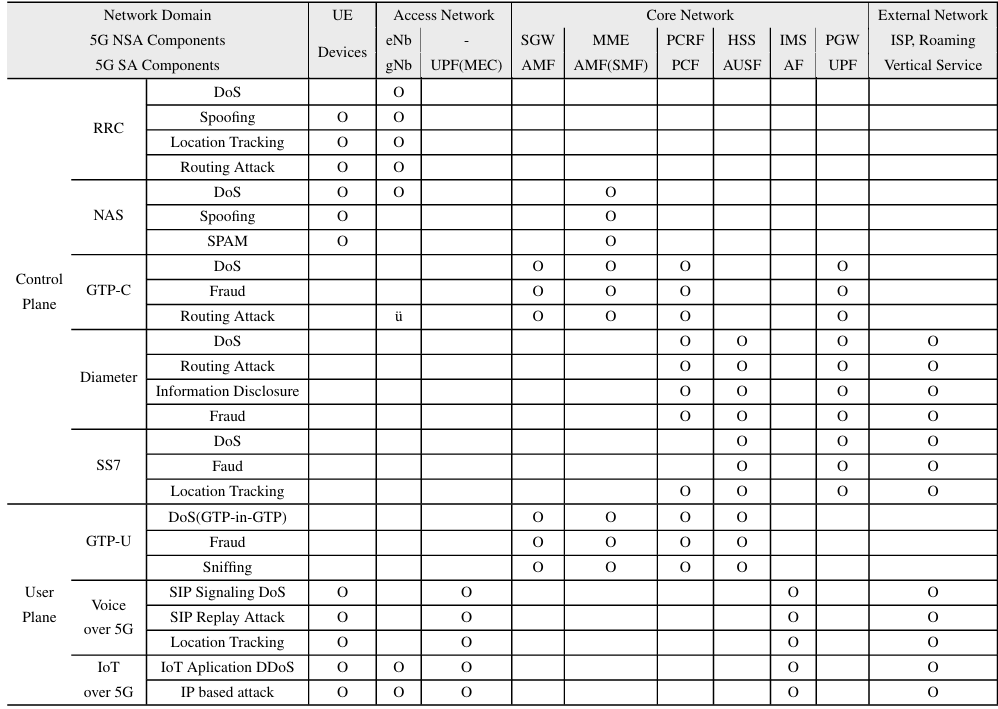
\includegraphics[width=\textwidth]{ATTACCHI.png}
	\caption{Classification of 5G Threat based network protocol}\label{fig:attacco}
	\texttt{Source: 5G core network security issues and attack classification from
		network protocol perspective, 2020}
\end{figure}

%--------------------------------------------------------------------------
\section{Conclusions}
La tecnologia 5G rappresenta una delle ultime frontiere nel campo delle
comunicazioni senza fili. Essa ha il potenziale di rivoluzionare molte attività
umane e il nostro modo di concepire le comunicazioni moderne, grazie a elevate
velocità di trasmissione, bassa latenza e un alto throughput. Tuttavia, con
l'avanzamento della tecnologia mobile, si sviluppano anche nuove minacce che
possono compromettere la sicurezza di queste reti. In questo articolo, sono
state analizzate le principali vulnerabilità associate al 5G. Molte di queste
vulnerabilità sono ereditate dal 4G, mentre altre sono completamente nuove. La
ricerca sulla sicurezza e l'identificazione di soluzioni innovative
rappresentano un compito cruciale per tutti gli attori coinvolti, dai fornitori
di servizi di rete a coloro che definiscono i protocolli di comunicazione.
Questo diventa particolarmente necessario, considerando che il 5G è sempre più
fondamentale per settori della vita quotidiana che possono diventare
estremamente delicati se non gestiti correttamente, come la telemedicina e i
veicoli a guida autonoma. L’evoluzione della cybersecurity nel contesto del 5G
non è solo una risposta alle minacce esistenti, ma anche una sfida per
prevedere e mitigare rischi futuri, considerando la crescente interconnessione
globale. Tecnologie chiave come l'intelligenza artificiale e il machine
learning offrono un potenziale significativo per migliorare la protezione delle
reti, identificando in tempo reale minacce sofisticate e attacchi su larga
scala. Inoltre, la crittografia deve evolversi per far fronte a nuove forme di
attacco, inclusi quelli che potrebbero emergere dall’uso di computer
quantistici. Guardando al futuro, è chiaro che la sicurezza del 5G diventerà un
aspetto sempre più centrale, soprattutto con l'incremento dei dispositivi IoT
connessi e l’utilizzo del 5G in infrastrutture critiche. Senza una protezione
adeguata, le conseguenze potrebbero essere devastanti, mettendo a rischio non
solo la privacy degli utenti, ma anche la stabilità dei sistemi economici e
sociali. La cooperazione internazionale, lo sviluppo di nuove tecnologie e la
definizione di standard sempre più stringenti saranno essenziali per garantire
che il 5G sia non solo un motore di progresso, ma anche una piattaforma sicura
per le generazioni future. \clearpage \appendix
\section{Termini da ricordare}
\begin{itemize}
	\item \textbf{\hypertarget{MIMO}{Massive MIMO}}: I sistemi wireless Multiple Input Multiple Output
	      sfruttano più antenne di trasmissione e ricezione per aumentare la capacità di rete,
	      migliorando il throughput dei dati e servendo un maggior numero di utenti. MIMO suddivide
	      il segnale in sottosegnali a bassa velocità, trasmessi su antenne spazialmente separate
	      sullo stesso canale di frequenza. Grazie alla propagazione su percorsi multipli, il
	      ricevitore separa i segnali in flussi paralleli per recuperare il segnale originale.
	      MIMO aumenta la capacità del canale senza consumare ulteriore larghezza di banda o
	      potenza e la velocità può crescere aggiungendo più antenne. Nel 5G, la tecnologia
	      Massive MIMO va oltre la configurazione $2 \times 2$ del 4G, utilizzando numerosi
	      flussi simultanei per aumentare la capacità di rete e l'efficienza spettrale.
	      L'array di antenne più grande permette un'elaborazione coerente del segnale, adattandosi
	      velocemente ai cambiamenti del canale di propagazione~\cite{Kathavate2021Critical}.

	\item \textbf{\hypertarget{mmWave}{mmWave}}: Le comunicazioni ad onde millimetriche
	      si rifereiscono all'uso di onde elettromagnetiche molto elevate, tipicamente comprese
	      tra \textit{30 GHz e 300GHz}. Questo onde sono chiamate millimetriche perchè la loro
	      lunghezza d'nda varia tra 1mm e 30mm, che sono molto più corte rispetto alle ond radio
	      tradizionalmente usate. Esse permetono velocità molto elevate e basssa latenza, ma hanno
	      una portata limitata e scarsa capacità di penetrazione, richiedendo infrastrutture dense
	      come small cells e tecnologie avanzate come il beamforming. Utilizzate insieme
	      a frequenze più basse per garantire una copertura completa,
	      le mmWave sono cruciali per migliorare la capacità delle
	      reti in aree ad alta densità di utenti.

	\item \textbf{\hypertarget{EAP-AKA}{EAP-AKA}}: è un protocollo di autenticazione progettato
	      per consentire l'autenticazione sicura tra un dispositivo mobile e una rete, basato
	      sul concetto di chiavi simmetriche. Quando un dispositivo, desidera connettersi a
	      una rete, invia una richiesta di autenticazione utilizzando un \texttt{SUCI},
	      una versione cifrata del suo identificatore permanente, il \texttt{SUPI}, consentendo
	      alla rete di identificare il dispositivo senza rivelare l’identità reale dell’utente
	      e garantendo la sua privacy. La rete, ricevuta la richiesta, utilizza il SUCI per
	      accedere alle credenziali memorizzate nel database dell’\texttt{ARPF}, dove è custodita
	      la chiave segreta \texttt{K}, condivisa tra il dispositivo e la rete; se viene scelto
	      il protocollo \texttt{EAP-AKA}, la rete avvia il processo di autenticazione generando
	      una \texttt{sfida} per il dispositivo composta da tre elementi: un numero casuale
	      \texttt{(RAND)}, un messaggio di autenticazione \texttt{(AUTN)} e la risposta attesa
	      \texttt{(XRES)}, che vengono inviati al dispositivo. Questo verifica il valore
	      \texttt{AUTN} utilizzando la chiave \texttt{K} nella sua \texttt{USIM}, e, se
	      l'\texttt{AUTN} è valido, calcola una risposta \texttt{(RES)} basata su \texttt{RAND}
	      e la chiave \texttt{K}, quindi la invia alla rete, che confronta la \texttt{RES}
	      ricevuta con la \texttt{XRES} generata in precedenza; se corrispondono,
	      l’autenticazione ha successo e entrambe le parti hanno verificato l'identità reciproca.
	      Successivamente, si genera la chiave di sessione, derivata dalla chiave \texttt{K}
	      e dai materiali generati nella sfida, con chiavi come \texttt{CK}
	      (per la cifratura dei dati) e \texttt{IK} (per l’integrità dei messaggi), essenziali
	      per proteggere le comunicazioni. Una volta completato il processo di autenticazione
	      e derivate le chiavi di sessione, il dispositivo e la rete possono iniziare a scambiare
	      dati in modo sicuro, sapendo che le comunicazioni sono protette
	      da solide misure di sicurezza.

	\item \textbf{\hypertarget{5G AKA}{5G AKA}}: Il processo \texttt{5G AKA} inizia con l'invio,
	      da parte del dispositivo, di una richiesta di autenticazione alla rete tramite il \texttt{SUCI},
	      una versione cifrata del \texttt{SUPI}, che protegge l'identità dell'utente durante la registrazione.
	      La rete riceve questa richiesta e la invia al database delle credenziali,
	      che contiene la chiave segreta \texttt{K} condivisa tra il dispositivo e la rete.
	      Se viene scelto il protocollo \texttt{5G AKA}, la rete genera una \texttt{sfida}
	      composta da un numero casuale \texttt{(RAND)}, un'autenticazione temporanea \texttt{(AUTN)}
	      e una risposta attesa \texttt{(XRES)}, che vengono inviati al dispositivo.
	      Il dispositivo, usando la chiave \texttt{K} memorizzata nella \texttt{USIM},
	      verifica l'\texttt{AUTN} per confermare l'identità della rete;
	      se la verifica è valida, calcola una risposta \texttt{(RES)} basata su \texttt{RAND} e \texttt{K},
	      che viene poi inviata alla rete. La rete confronta la \texttt{RES} con la \texttt{XRES} generata in precedenza,
	      e se corrispondono, l'autenticazione ha successo.\@
	      A questo punto, vengono generate le chiavi di sessione per la cifratura
	      e l'integrità delle comunicazioni, garantendo la sicurezza dei dati trasmessi.
	      Una caratteristica importante del \texttt{5G AKA} è il rafforzamento della privacy dell'utente,
	      grazie alla separazione delle chiavi di cifratura e integrità e a meccanismi più robusti
	      per prevenire attacchi di tracciamento e correlazione delle identità,
	      migliorando significativamente la sicurezza rispetto alle generazioni precedenti.\@

	\item \textbf{\hypertarget{PLMN}{PLMN (Public Land Mobile Network)}}:
	      È una rete mobile pubblica terrestre. Un PLMN è una rete mobile che fornisce servizi di
	      comunicazione mobile al pubblico. Ogni operatore mobile ha il proprio PLMN identificato
	      da un codice univoco, che consente ai dispositivi di identificare e connettersi a quella rete.

	\item \textbf{FBMC}\hypertarget{FBMC}{}: Il Filter Bank Multicarrier (FBMC) è una tecnica di
	      modulazione che divide un segnale in più sottocanali, applicando filtri per ridurre
	      le interferenze tra questi, migliorando così l'efficienza spettrale rispetto all'OFDM.\@

	\item \textbf{FullDuplex}\hypertarget{FullDuplex}{}:Il full duplex è una modalità di comunicazione
	      in cui i dati possono essere trasmessi e ricevuti contemporaneamente tra due dispositivi
	      o punti. In altre parole, entrambe le parti possono inviare e ricevere informazioni allo
	      stesso tempo, senza dover aspettare che una delle due abbia finito di trasmettere.

	\item \textbf{Ultra Dense Networking}\hypertarget{UDN}{}:L'Ultra Dense Networking (UDN) è una
	      architettura di rete progettata per migliorare la capacità e la copertura della rete
	      in ambienti ad alta densità di utenti o dispositivi.DN si basa sull'idea di aumentare
	      il numero di celle o piccole stazioni base (small cells) in un'area geografica,
	      riducendo la distanza tra queste stazioni e i dispositivi connessi. Questo riduce il
	      carico su ogni singola stazione base, migliorando la capacità di banda e la qualità
	      del segnale.

	\item \textbf{Software-Defined Networking}\hypertarget{SDN}{}:  Software-Defined Networking (SDN)
	      è un approccio alla gestione delle reti che separa il piano di controllo (control plane)
	      dal piano dati (data plane). Tradizionalmente, i router e gli switch svolgono sia il
	      compito di instradare il traffico (piano dati) che di decidere come farlo
	      (piano di controllo). SDN sposta il piano di controllo in un'entità software centrale
	      chiamata \texttt{controller}, che ha una visione globale della rete e può programmare
	      dinamicamente come i pacchetti devono essere gestiti dagli switch, semplificando la
	      gestione della rete e migliorandone l'agilità.

	\item \textbf{Network Function Virtualization}\hypertarget{NFV}{}: La Network Function
	      Virtualization (NFV) è una tecnologia che virtualizza le funzioni di rete, come firewall,
	      router, load balancer e altri dispositivi di rete, su server standard,
	      eliminando la necessità di hardware specializzato. NFV consente di distribuire e gestire
	      le funzioni di rete come software, migliorando la scalabilità, la velocità di
	      implementazione e riducendo i costi.

	\item \textbf{\hypertarget{S-TMSI}{S-TMSI}}: è un identificatore temporaneo
	      utilizzato nelle reti 4G LTE e 5G per rappresentare un abbonato senza rivelarne
	      l'IMSI (International Mobile Subscriber Identity).
	      Esso viene generato dalla rete e cambia periodicamente,
	      riducendo il rischio di tracciamento e attacchi informatici.

	\item \textbf{\hypertarget{RRC}{RRC}}: RRC è un protocollo fondamentale
	      nel piano di controllo delle reti mobili ed è responsabile della gesione delle
	      connessioni radio tra l'utente e la rete. Le principali funzioni
	      del protocllo RRC includono: l'instaurazione e il rilascio della connesione radio,
	      la gestione della mobilità, il controllo qalità  e la trasmissione di informazioni
	      di confgurazione e segnalazione.

	\item \textbf{eNB}\hypertarget{eNB}{}: Rappresenta il  nodo di accesso radio delle reti
	      \texttt{4G LTE}.\@ eNB è responsabile della trasmissione e ricezione dei segnali radio
	      tra l'utente finale e la rete core \texttt{LTE} e ha funzioni di gestione delle risorse radio,
	      codifica e decodifica, controllo di potenza, gestione della mobilità e dellos cheduling dei dati.

	\item \textbf{gNB}\hypertarget{gNB}{}: Il next generation Node B è l'elemento
	      della rete di accesso radio nella tecnologia 5G.
	      Oltre a supportare i tradizionali servizi a banda larga, il gNodeB consente
	      funzionalità avanzatate come le comunicazioni massive per dispositive IoT e La
	      gestione del traffico con qualità del servizio variabile in base alle
	      esigenze dell'applicazione.

	\item \hypertarget{IMSI}{\textbf{IMSI}}: International Mobile Subscriber Identity
	      è un numero identificativo univoco,
	      composto da 15 cifre associato a ciascun abbonato nella rete mobili.
	      Questo numero è utilizzato per identificare e autenticare un utente all'interno
	      di una rete mobile.\@ \texttt{IMSI} è memorizzato nella scheda SIM e include il
	      codice del paese \texttt{(MCC)},
	      il codice dell'operatore \texttt{(MNC)}
	      e un numero identificativo dell'abbbonato \texttt{(MSIN)}.

	\item \hypertarget{SDR}{SDR}: Un dispositivo SDR (Software-Defined Radio)
	      è una radio in cui gran parte delle operazioni di elaborazione del segnale,
	      come modulazione e demodulazione, viene eseguita tramite software anziché hardware fisso.
	      Questo permette di adattare il dispositivo a diverse frequenze e protocolli radio
	      semplicemente aggiornando il software, rendendolo estremamente flessibile e versatile
	      per applicazioni come telecomunicazioni, ricerca e analisi di sicurezza.

	\item \textbf{\hypertarget{RTP}{RTP}}: Il Real-time Transport Protocol (RTP) è un protocollo
	      di rete utilizzato per la trasmissione di dati in tempo reale, come voce e video, su reti IP.\@

	\item \textbf{\hypertarget{GTP}{GTP}}: è un protocollo è routing. Il suo scopo è quello di trasportare dati tra
	      diversi nodi rete in maniera efficiente.

	\item \textbf{\hypertarget{NAS}{NAS}}: Gestisce la comunicazione tra il dispositivo dell'utente e il
	      core network, occupandosi di autenticazione e registrazione, assicurando che solo i dispositivi
	      autorizzati accedano alla rete. Inoltre, si occupa della mobilità, consentendo agli utenti di
	      passare da una cella all'altra senza interruzioni. Gestisce anche le sessioni di dati, stabilendo
	      e terminando le connessioni e mantenendo la qualità del servizio.

	\item \textbf{\hypertarget{MME}{MME}}: L'Mobility Management Entity (MME) è un componente software nel
	      core network delle reti mobili 4G e 5G, responsabile della gestione della mobilità degli utenti
	      e della segnalazione. Svolge funzioni chiave come l'autenticazione degli utenti, la gestione
	      delle sessioni,
	      il monitoraggio della posizione e l'instradamento delle richieste di servizio verso
	      altre entità di rete. L'MME comunica con dispositivi terminali e altri elementi
	      della rete utilizzando protocolli come NAS (Non Access Stratum) e
	      GTP (GPRS Tunneling Protocol).
\end{itemize}
\clearpage
\printbibliography\end{document}
